\begin{frame}
  \begin{center}
    {\huge GloVe: Global Vectors for Word Representation
    } \\
    Pennington,Socher,Manning
  \end{center}
\end{frame}
%%%%%%%%%%%%%%%%%%%%%%%%%%%%%%%%%%%%%%%%%%%%%%%%%%

\begin{frame}{Introduction - What is a Word Vector?}
  \begin{itemize}
    %% Word vectors capture linguistic regularities in a simple manner.
  \item A mathematical representation of words.
    %% conventional way - one hot repr lead to data sparsity, does not take word relationships into account
  \item Representation captures some form of ``related-ness''.
    \begin{figure}
      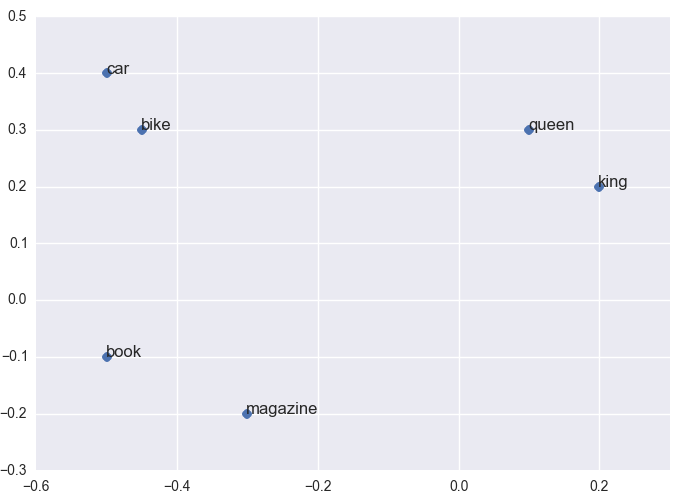
\includegraphics[scale=0.35]{images/wordvec.png}
      \caption{From}
    \end{figure}    
  \end{itemize}
\end{frame}


%%%%%%%%%%%%%%%%%%%%%%%%%%%%%%%%%%%%%%%%%%%%%%%%%%
\begin{frame}{Generating Vector Representations}
  Word vectors can be generated in the following ways:
  \begin{itemize}[<+->]
  \item Cooccurence Matrix Factorization~\cite{Deerwester} % HAL,LSA the name of the game is compute co-occurence
    % fully unsupervised!
  \item Learn representation from Local Context ~\cite{Mikolov13a}.%
  \item Sometimes just using the explicit context representation suffices ~\cite{Levy14}.
    %% Sometimes these methods end-up modeling the same objective (skip-gram).
    %% what abt random sampling
  \end{itemize}
  \visible<4>
  {This paper proposes another way of obtaining word vectors via matrix factorization.}
  %% They claim that their model combines advantages of both global and local? (??)
\end{frame}

%%%%%%%%%%%%%%%%%%%%%%%%%%%%%%%%%%%%%%%%%%%%%%%%%%
\begin{frame}{Structure in Word Vector Spaces}
  The configuration of the vectors encode relationships between words.
  \begin{align*}
    v(king) - v(man) + v(woman) \approx v(queen)
  \end{align*}
  \pause
  \visible<2->
      {
        \begin{figure}
          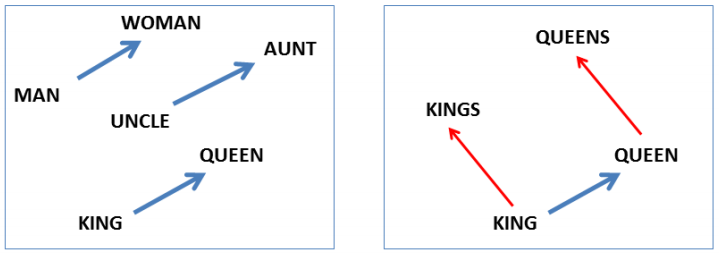
\includegraphics[scale=0.35]{images/mikolov.png}
          \caption{From}
        \end{figure}
      }
      %% No explanation was given in the original papers.
      %% {\footnotesize Remarkably, training such a lexical model induces word repr. with striking semantic and syntactic properties---\cite{Mikolov13a}} \\
      %% Levy showed that tranditional methods like count sparse contexts can perform equally well.
      %% {\footnotesize ... traditional word similarities can perform just as well as neural embeddings ---\cite{Levy14}} \\
      %% talk about Dont Count Predict paper
      \visible<3>
      {This paper claims to explicitly model properties needed for achieving the above effect.}
\end{frame}

%% \begin{frame}{Problems}
%%   Global Matrix Factorization Methods are prone to ill-effects of predominance of function words.
%% \end{frame}



%% %%%%%%%%%%%%%%%%%%%%%%%%%%%%%%%%%%%%%%%%%%%%%%%%%%
%% \begin{frame}{What's new in this paper?}
%%   \begin{itemize}
%%   \item They claim their objective is explicitly modelling vector structure to facilitate linear 
%%   \end{itemize}
%% \end{frame}


%%%%%%%%%%%%%%%%%%%%%%%%%%%%%%%%%%%%%%%%%%%%%%%%%%
\begin{frame}{GloVe Model}
  \begin{figure}
    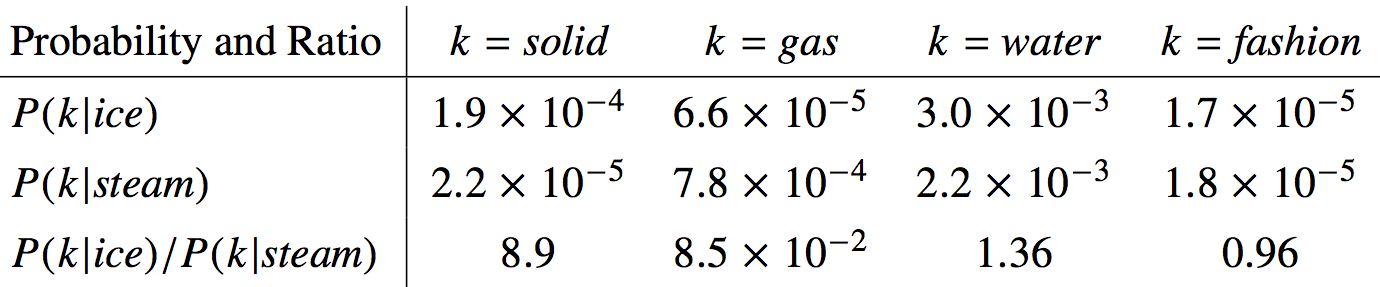
\includegraphics[scale=0.23]{images/glove_int.png}
  \end{figure}
  \visible<2>{
    \begin{align*}
      \frac{\Pr(k \mid king)}{\Pr(k \mid queen)} \approx \frac{\Pr(k \mid man)}{\Pr(k \mid woman)}
    \end{align*}    
  }
\end{frame}

%%%%%%%%%%%%%%%%%%%%%%%%%%%%%%%%%%%%%%%%%%%%%%%%%%
\begin{frame}{GloVe Model}
  \begin{align*}
    %% & \Pr(\text{word j appears in context of word i}) = \Pr_{ij} \\
    & \Pr_{ij} \propto \exp(\dotprod{w_i}{\tilde{w}_j}) \tag{log-bilinear model}
  \end{align*}
  \pause
  \begin{align*}
    & w_i^T\tilde{w_j} + \tilde{b_j} = \log X_{ij} - \log X_{i} \tag{$\Pr_{ik}=\frac{X_{ik}}{X_i}$} \\
    %% & \frac{\Pr_{ik}}{\Pr_{jk}}=\exp(\dotprod{w_i -w_j}{\tilde{w}_k}) \\
    %% & \log \Pr_{ik} - \log\Pr_{jk} = \dotprod{w_i -w_j}{\tilde{w}_k}\\
    & w_i^T\tilde{w_j} +b_i + \tilde{b_j} = \log X_{ij}
  \end{align*}
  \pause
  We can minimize 
  \begin{align*}
    & \sum_{i=1,j=1}^V \left( w_i^T\tilde{w_j} +b_i + \tilde{b_j} - \log X_{ij} \right)^2
  \end{align*}
  \pause
  %% note the similarity with matrix factorization
  But wait!
\end{frame}

%%%%%%%%%%%%%%%%%%%%%%%%%%%%%%%%%%%%%%%%%%%%%%%%%%
\begin{frame}{GloVe Model - Introduce Weighted Cost}
  \begin{align*}
    & J = \sum_{i=1,j=1}^V \alert{f(X_{ij})} \left( w_i^T\tilde{w_j} +b_i + \tilde{b_j} - \log X_{ij} \right)^2
  \end{align*}
  $f$ should not overweight rare and too-frequent occurences.

  \visible<2>{
    \begin{figure}
      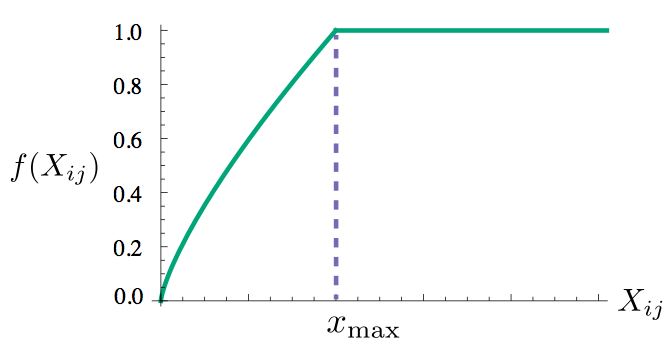
\includegraphics[scale=0.27]{images/weighting.png}
      \caption{From}
    \end{figure}
  }
  
\end{frame}

%%%%%%%%%%%%%%%%%%%%%%%%%%%%%%%%%%%%%%%%%%%%%%%%%%
%% \begin{frame}{Training}
%% \begin{itemize}
%% \item Vector Length:
%% \item Context Size: 
%% \item Corpus Size: nothing supriszing
%% \end{itemize}
%% \end{frame}

%%%%%%%%%%%%%%%%%%%%%%%%%%%%%%%%%%%%%%%%%%%%%%%%%%
\begin{frame}{Model Analysis}
  \begin{itemize}
  \item Vector Length:
  \item Context Size: 
  \item Corpus Size: nothing suprising
  \item Model trained on smaller wikipedia corpus( 1.6B tokens) does better on semantic task than model trained on larger corpus like gigaword (4.3B tokens)
  \item Idea: instead of using only word vector $w$, use $w+c$, where $c$ is the context vector (significant improvement in semantic task). This can be used for other models as well.
  \end{itemize}
\end{frame}

%%%%%%%%%%%%%%%%%%%%%%%%%%%%%%%%%%%%%%%%%%%%%%%%%%
\begin{frame}{Evaluation}
  \begin{itemize}[<+->]
  \item Semantic Relatedness % (Google Dataset) % intrinsic
    \begin{itemize}
    \item \textsc{Athens} is to \textsc{Greece} as \textsc{Berlin} is to ? (\textsc{Germany})
    \item \textsc{Putin} is to \textsc{Russia} as \textsc{Sarkozy} is to ? (\textsc{France})
    \end{itemize}
  \item Syntactic Relatedness % (Google dataset, MSR dataset) % intrinsic
    \begin{itemize}
    \item \textsc{Car} is to \textsc{Cars} as \textsc{Family} is to ? (\textsc{families})
    \item \textsc{Carry} is to \textsc{Carried} as \textsc{Go} is to ? (\textsc{went})
    \end{itemize}
  \item NER 
    \begin{itemize}
    \item User word vectors as continuous features in a NER system.
    \end{itemize}
  \end{itemize}
\end{frame}

%%%%%%%%%%%%%%%%%%%%%%%%%%%%%%%%%%%%%%%%%%%%%%%%%%
\begin{frame}{Results}
  \begin{figure}
    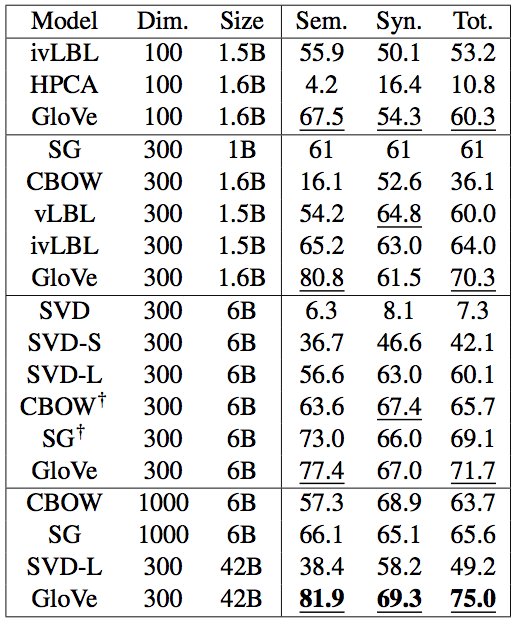
\includegraphics[scale=0.27]{images/results1.png}
    \caption{From}
  \end{figure}
\end{frame}

%%%%%%%%%%%%%%%%%%%%%%%%%%%%%%%%%%%%%%%%%%%%%%%%%%
\begin{frame}{Results}
  \begin{figure}
    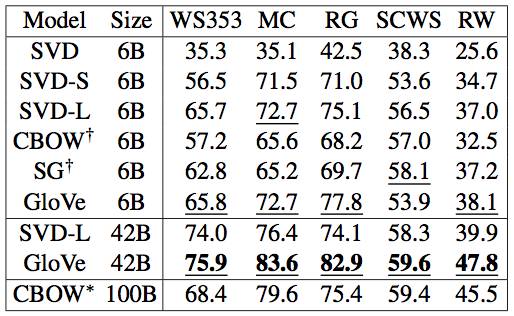
\includegraphics[scale=0.27]{images/results2.png}
    \caption{From}
  \end{figure}
\end{frame}

%%%%%%%%%%%%%%%%%%%%%%%%%%%%%%%%%%%%%%%%%%%%%%%%%%
\begin{frame}{Results}
  \begin{figure}
    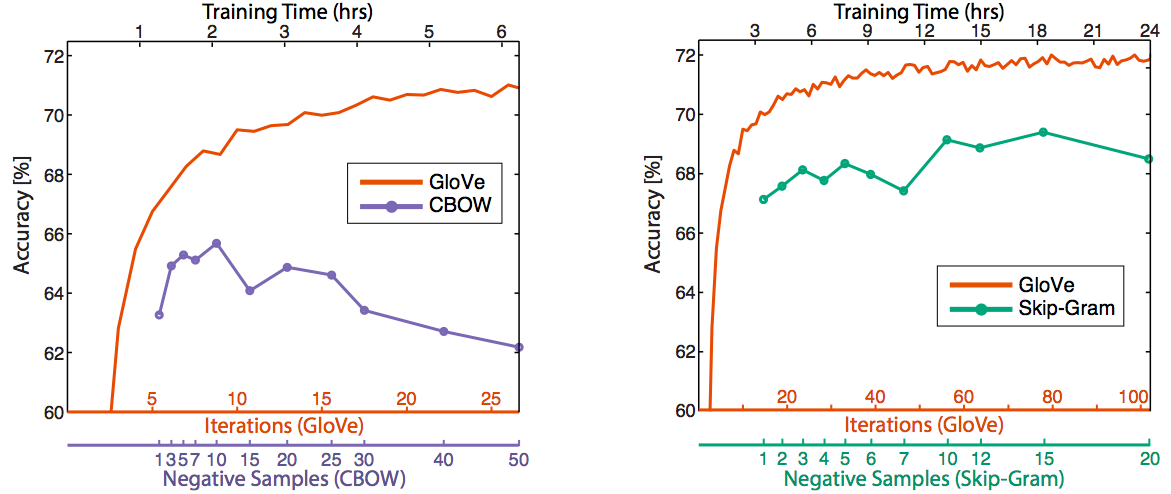
\includegraphics[scale=0.27]{images/gloveVSword2vec.png}
    \caption{From}
  \end{figure}
\end{frame}

%%%%%%%%%%%%%%%%%%%%%%%%%%%%%%%%%%%%%%%%%%%%%%%%%%
\begin{frame}{Results}
  \begin{figure}
    \centering
    \begin{subfigure}[b]{0.33\textwidth}
      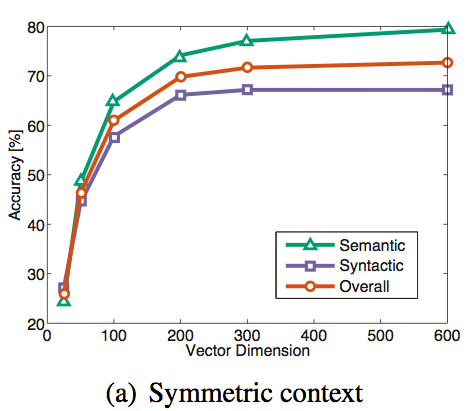
\includegraphics[width=\textwidth]{images/analogy1.png}
    \end{subfigure}%
    \begin{subfigure}[b]{0.33\textwidth}
      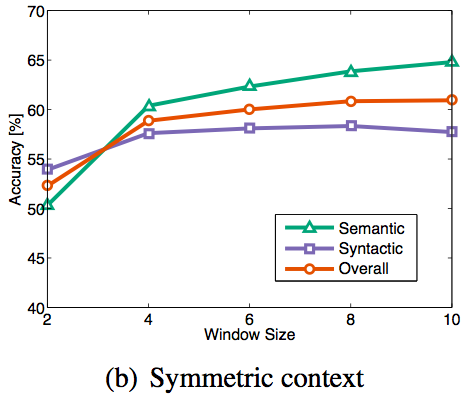
\includegraphics[width=\textwidth]{images/analogy2.png}
    \end{subfigure}%
    \begin{subfigure}[b]{0.33\textwidth}
      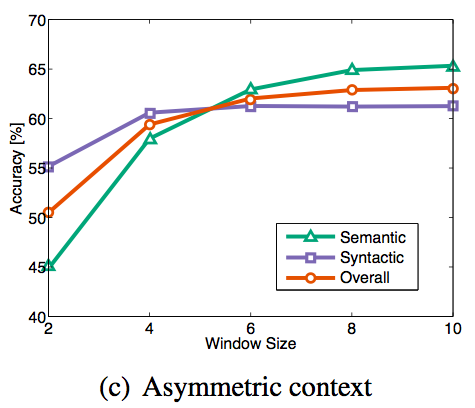
\includegraphics[width=\textwidth]{images/analogy3.png}
    \end{subfigure}%
  \end{figure}
\end{frame}


\begin{frame}
  new ideas from Turian Ratinov Bengio,
  curriculum training strategy?
  liang's preprocessing
  connotation vs denotation
  distributional vs distributed
  exp not done MSR dataset,
  batch restriction for glove vs online training for skip gram
\end{frame}
